\documentclass[11pt,a4paper]{jsarticle}
%
\usepackage{amsmath,amssymb}
\usepackage{bm}
\usepackage[dvipdfm]{graphicx}
\usepackage{ascmac}
\usepackage{float}
%
\setlength{\textwidth}{\fullwidth}
\setlength{\textheight}{39\baselineskip}
\addtolength{\textheight}{\topskip}
\setlength{\voffset}{-0.5in}
\setlength{\headsep}{0.3in}
%
\newcommand{\divergence}{\mathrm{div}\,}  %ダイバージェンス
\newcommand{\grad}{\mathrm{grad}\,}  %グラディエント
\newcommand{\rot}{\mathrm{rot}\,}  %ローテーション
%
\pagestyle{myheadings}
\markright{}
\begin{document}
%
%
\section*{補足資料}
\begin{itemize}
\item PPM (Park Power Management)
\end{itemize}
\begin{flushleft}
ドイツ電力会社E-onが発電自供者に出力制限指令を与えて風力から系統に流入する電力を抑制するために開発された制御機能

PPMの主な性能

 ・最大出力を制限可能

 ・目標値(パーク指令)に対して変動が残るため、若干の制御裕度が必要

 ・上ブレについては補償が可能

   ※ただし利用率の低下を招く

 ・下ぶれについては対策不可

\end{flushleft}
\begin{figure}[h]
\centering
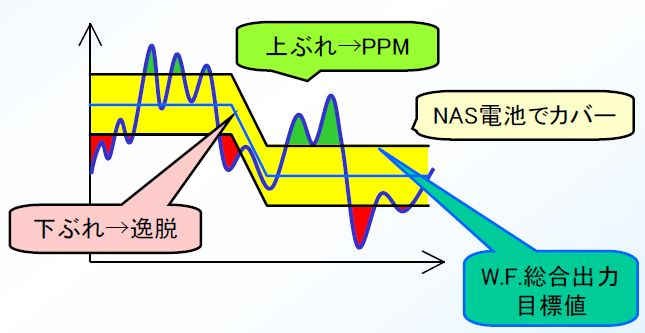
\includegraphics[width=6cm,bb=0 0 645 333]{WS000003.jpg}
\caption{PPMの性能}
\label{image_sample}
\end{figure}

%
%
\end{document}